\section{Calculus with Parametric Curves}
\begin{itemize}
    \item Parametric curves do not need to be functions. As a result, they can have an ordinary tangent, no tangent, or more than one tangent at the same point.
    \item We can find the secant line of a parametric curve via:
    \begin{equation}
        m_\text{secant} = \frac{y(t_0+h)-y(t_0)}{x(t_0+h)-x(t_0)}
    \end{equation}
    We can divide both numerator and denominator by $h$ to get:
    \begin{equation}
        \frac{\frac{y(t_0+h)-y(t_0)}{h}}{\frac{x(t_0+h)-x(t_0)}{h}} \implies \frac{y'(t_0)}{x'(t_0)}
    \end{equation}
    where we took the limit as $h\to 0$.
    \item We could also have derived this using the chain rule:
    \begin{equation}
        \frac{dy}{dx} = \frac{dy}{dt}\cdot \frac{dt}{dx} = \frac{dy}{dt}\left(\frac{dx}{dt}\right)^{-1}
    \end{equation}
    \item If $x'(t_0)=0$, then $x=x_0$ is a vertical tangent and if $y'(t_0)=0$, then we have $y=y_0$ and have a horizontal tangent. If $x'=y'=0$, then we can't read any information from it.
    \begin{example}
        Consider the example $x(t) = \sin(2t)$ and $y(t)=\sin t$ with $t\in [0,2\pi]$. We have $x'(t) = 2\cos 2t$ so we can find the vertical tangents by setting $2\cos(2t) = 0$ to get:
        \begin{equation}
            t \in \{\frac{\pi}{4}, \frac{3\pi}{4}, \frac{5\pi}{4}, \frac{7\pi}{4}\} \implies \left(1,\frac{1}{\sqrt{2}}\right)\,\left(-1,\frac{1}{\sqrt{2}}\right)\,\left(1,-\frac{1}{\sqrt{2}}\right)\,\left(-1,-\frac{1}{\sqrt{2}}\right)
        \end{equation}
        For horizontal tangents, we have $y'(t) = \cos t \implies \cos t = 0$ which gives:
        \begin{equation}
            t \in \{\frac{\pi}{2}, \frac{3\pi}{2}\} \implies (0,1) (0,-1)
        \end{equation}
        At $t=0$, we also have $x(0)=y(0)=0$. We can determine the tangent at this point as:
        \begin{equation}
            m_\text{tangent} = \frac{y'(0)}{x'(0)} = \frac{1}{2}
        \end{equation}
        However notice that at $t=\pi$, we have $x(\pi)=y(\pi)=0$ as well so this point has another tangent:
        \begin{equation}
            m_\text{tangent} = \frac{y'(\pi)}{x'(\pi)} = -\frac{1}{2}
        \end{equation}
        At this point we can sketch out the conditions we found on the graph and draw out curve:
        \begin{center}
            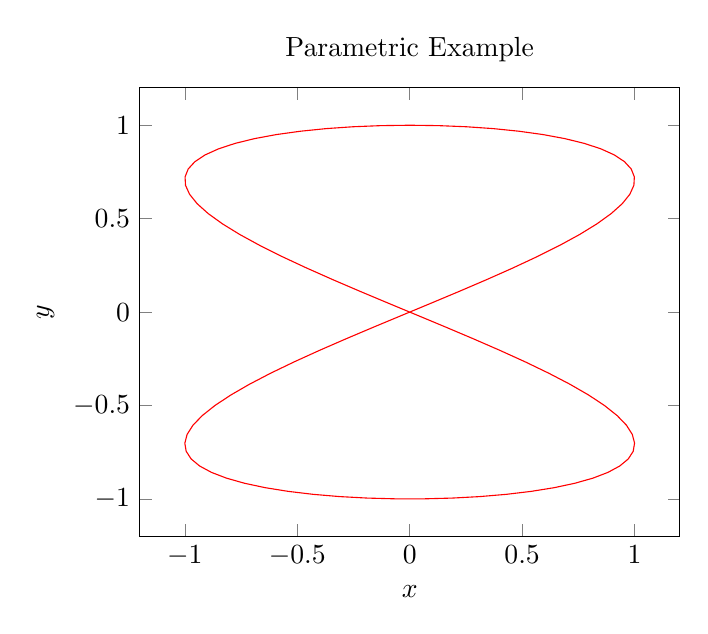
\begin{tikzpicture}
            \begin{axis}[
            trig format plots=rad,
            legend pos=outer north east,
            title=Parametric Example,
            axis lines = box,
            xlabel = $x$,
            ylabel = $y$,
            ]
            \addplot [domain=0:2*pi, samples=100, red] ({sin(2*x)}, {cos(x)});
            \end{axis}
            \end{tikzpicture}
        \end{center}
    \end{example}
    \item We can determine the \textbf{area} of a parametric curve via:
    \begin{align}
        A = \int_{t_1}^{t_2}y(t)x'(t) \dd{t}
    \end{align}
    Letting $y=f(x) \implies y(t) = f(x(t))$ gives:
    \begin{align}
        A &= \int_{t_1}^{t_2} f(x(t))x'(t) \dd{t} \\ 
        &= \int_{a=x(t_1)}^{b=x(t_2)} f(x) \dd{x}
    \end{align}
    \item We can also determine the area of a closed curve:
    \begin{definition}
        A curve is traversed in the positive sense as $t$ increases, if the enclosed area is on the left (counterclockwise).
    \end{definition}
    The area of a closed loop is then:
    \begin{equation}
        A = \int_{t_4}^{t_3}y(t)x'(t)\dd{t} - \int_{t_4}^{t_5}y(t)x'(t)\dd{t} + \int_{t_3}^{t_2}y(t)x'(t)\dd{t} - \int_{t_1}^{t_2}y(t)x'(t)\dd{t}
    \end{equation}
    where $t_1$ represents the starting point on the bottom, $t_2$ is the rightmost point, $t_3$ is an arbitrary point on top, $t_4$ is the leftmost point, and $t_5$ is the endpoint that ends off as $t_1$. This gives:
    \begin{align}
        -\int_{t_3}^{t_4}y(t)x'(t)\dd{t} - \int_{t_4}^{t_5}y(t)x'(t)\dd{t} - \int_{t_2}^{t_3}y(t)x'(t)\dd{t} - \int_{t_1}^{t_2}y(t)x'(t)\dd{t}
    \end{align}
    or:
    \begin{equation}
        A = -\int_{t_1}^{t_5} y(t)x'(t) \dd{t}
    \end{equation}
    where $t_1$ and $t_5$ are the starting and ending points respectively. They can be arbitarrily chosen so long as the points they coorespond to are on top of each other.
    \item Similarly, we can also write the area as:
    \begin{equation}
        A = \int_{t_1}^{t_5} x(t) y'(t) \dd{t}
    \end{equation}
    \begin{example}
        Let us derive the area of an ellipse, parametized by:
        \begin{align}
            x &= a\cos \theta \\ 
            y &= b\sin\theta
        \end{align}
        for $\theta \in [0,2\pi]$. The area is then:
        \begin{align}
            A &= -\int_0^{2\pi} b\sin\theta (-a\sin\theta) d\theta \\ 
            &= ab\int_0^{2\pi} \sin^2\theta \dd{\theta} \\ 
            &= ab\left[\frac{1}{2}\theta - \frac{1}{4}\sin 2\theta\right]^{2\pi}_{0} \\ 
            &= \pi ab
        \end{align}
    \end{example}
    \item We can also determine the \textbf{arclength} of a parametric curve. We start with the summation:
    \begin{equation}
        s \simeq \sum \sqrt{\Delta x^2+\Delta y^2} \implies \int_{\alpha}^{\beta}\sqrt{x'(t)^2+y'(t)^2}\dd{t}
    \end{equation}
    Note that if we let $x=t$ and $y=f(t)=f(x)$, then we get:
    \begin{equation}
        s = \int_{\alpha}^{\beta}\sqrt{1+f'(x)^2}\dd{x}
    \end{equation}
    which is what we should expect.
    \begin{example}
        Suppose we have $x(\theta) = \theta\cos\theta$ and $y(\theta)=\theta\sin\theta$ for $\theta \in [0,2\pi]$, this gives an Archimedes Spiral:
        \begin{center}
            \begin{tikzpicture}
            \begin{axis}[
            trig format plots=rad,
            legend pos=outer north east,
            title=Parametric Example,
            axis lines = box,
            xlabel = $x$,
            ylabel = $y$,
            ]
            \addplot [domain=0:2*pi, samples=100, red] ({x*cos(x)}, {x*sin(x)});
            \end{axis}
            \end{tikzpicture}
        \end{center}
        We can determine the arclength via:
        \begin{align}
            s &= \int_0^{2\pi} \sqrt{(\cos\theta-\theta \sin\theta)^2 + (\sin\theta+\theta\cos\theta)^2} \dd{\theta} \\ 
            &= \int_0^{2\pi} \sqrt{1+\theta^2}\dd{\theta} \\ 
            &= \left[\frac{1}{2}\theta\sqrt{1+\theta^2}+\frac{1}{2}\ln\left|\theta+\sqrt{1+\theta^2}\right|\right]\Biggr|^{2\pi}_0 \\ 
            &= \pi\sqrt{1+4\pi^2} + \frac{1}{2}\ln\left(2\pi + \sqrt{1+4\pi^2}\right)
        \end{align}
    \end{example}
    \begin{idea}
        If we wish to find the speed, we have:
        \begin{equation}
            v = \frac{ds}{dt} = \sqrt{x'(t)^2+y'(t)^2}
        \end{equation}
        which comes from both the fundamental theorem of calculus, as well as from two-dimensional kinematics.
    \end{idea}
    \item The surface area can be written as:
    \begin{equation}
        A = \int_a^b 2\pi y \dd{s} = \int_a^b 2\pi y(t) \sqrt{x'(t)^2+y'(t)^2} \dd{t}
    \end{equation}
    \item What is the \textit{circumference of an ellipse?} If we try to carry out this calculation, we can parametize the ellipse as before:
    \begin{align}
        x &= a\sin\theta \\ 
        y &= b\cos\theta 
    \end{align}
    with $0 \le \theta \le 2\pi$ and the arclength as:
    \begin{align}
        s &= \int_0^{2\pi} \sqrt{a^2\cos^2\theta + b^2\sin^2\theta} \dd{\theta} \\ 
        &= \int_0^{2\pi} \sqrt{a^2(1-\sin 2\theta) + b^2\sin 2\theta} \dd{\theta} \\ 
        &= \int_0^{2\pi} a\sqrt{1- \epsilon^2 \sin^2\theta}
    \end{align}
    with $\epsilon \equiv \sqrt{\frac{a^2-b^2}{a^2}}$. Unfortunately, this is an elliptic integral of the second kind and has no analytic solution.
\end{itemize}